\documentclass[10pt]{beamer}

% ------------------------------------------------------------------------
% Carga de tu preámbulo personalizado (preamble.tex).
% Recuerda ponerlo en la misma carpeta para que \input funcione.
% ------------------------------------------------------------------------
\usetheme[progressbar=frametitle]{metropolis}
\usepackage{appendixnumberbeamer}
\usepackage{fancyvrb}
\usepackage{booktabs}
\usepackage[scale=2]{ccicons}
\usepackage{pgfplots}
\usepgfplotslibrary{dateplot}
\usepackage{type1cm}
\usepackage{lettrine}
\usepackage{ragged2e}
\usepackage{xspace}
\newcommand{\themename}{\textbf{\textsc{metropolis}}\xspace}
\usepackage{graphicx} % Allows including images
\usepackage{booktabs} % Allows the use of \toprule, \midrule and \bottomrule in tables
\usepackage[utf8]{inputenc} %solucion del problema de los acentos.
\usepackage{xcolor}
\definecolor{LightGray}{gray}{0.9}

\usepackage{minted}
\usemintedstyle{tango}
\newcommand{\mypyfile}[1]{\inputminted[linenos=true, fontsize=\footnotesize, frame=lines, framesep=5\fboxrule,framerule=1pt]{python}{#1}}

\setminted[python]{breaklines,frame=lines,framesep=2mm,baselinestretch=1.2,bgcolor=LightGray,linenos, fontsize=\footnotesize} % obeytabs=true, tabsize=2, showtabs=true}

%%%%%%%%%%%%%%%%%%%%%%%%%%%%%%%%%%%%%%%%%%%%%%%%%%%%%%%%%%%%%%%%%%%%%%%%%%%%%%%%%%%%%%
\setbeamercolor{progress bar}{fg=blue!50!black,bg=white!50!black}
\setbeamercolor{title separator}{fg=red!50!black,bg=white!50!black}
\setbeamercolor{frametitle}{fg=white!80!black,bg=red!50!black}
\title[PCFI161]{Programaci\'on para F\'isica y Astronom\'ia}
\subtitle{Departamento de Física.}

\newcommand{\myfront}{
\author[PCFI161]{Corodinadora: C Loyola \\ Profesoras/es C Loyola / C Femenías / Y Navarrete / C Ruiz}
\institute[UNAB]{Universidad Andrés Bello}
\date{Primer Semestre 2025}
}

\titlegraphic{%
  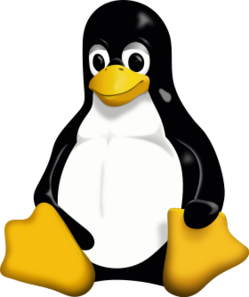
\includegraphics[width=.08\textwidth]{logo-tux.png}\hfill
  
\includegraphics[width=.3\textwidth]{logo-unab.png}\hfill
  
\includegraphics[width=.08\textwidth]{logo-python.png}
}

\makeatletter
\setbeamertemplate{title page}{
  \begin{minipage}[b][\paperheight]{\textwidth}
    \vfill%
    \ifx\inserttitle\@empty\else\usebeamertemplate*{title}\fi
    \ifx\insertsubtitle\@empty\else\usebeamertemplate*{subtitle}\fi
    \usebeamertemplate*{title separator}
    \ifx\beamer@shortauthor\@empty\else\usebeamertemplate*{author}\fi
    \ifx\insertdate\@empty\else\usebeamertemplate*{date}\fi
    \ifx\insertinstitute\@empty\else\usebeamertemplate*{institute}\fi
    \vfill
    \ifx\inserttitlegraphic\@empty\else\inserttitlegraphic\fi
    \vspace*{1cm}
  \end{minipage}
}
\makeatother


\makeatletter
\setlength{\metropolis@titleseparator@linewidth}{2pt}
\setlength{\metropolis@progressonsectionpage@linewidth}{2pt}
\setlength{\metropolis@progressinheadfoot@linewidth}{2pt}
\makeatother


\begin{document}

% ------------------------------------------------------------------------
% Portada de la Presentación
% ------------------------------------------------------------------------
\myfront{}

% ------------------------------------------------------------------------
% Slide 1: Título de la Sesión
% ------------------------------------------------------------------------
\begin{frame}
  \titlepage
  % Ejemplo:
  % \title{Semana 12 - Sesión 1 (Sesión 23): Lanzamiento de Proyectos y Nuevas Herramientas}
\end{frame}

% ------------------------------------------------------------------------
% Slide 2: Índice / Tabla de Contenidos
% ------------------------------------------------------------------------
\begin{frame}
  \frametitle{Resumen - Semana 12, Sesión 1 (Sesión 23)}
  \tableofcontents
\end{frame}

% ------------------------------------------------------------------------
% Configuración de bloques
% ------------------------------------------------------------------------
\metroset{block=fill}

% ----------------------------------------------------------------------------------------
% SECCIÓN 1: Introducción y Conexión con la Semana 11
% ----------------------------------------------------------------------------------------
\section{Introducción y Repaso}

% ------------------------------------------------------------------------
% Slide 3: Conexión con la Semana 11
% ------------------------------------------------------------------------
\begin{frame}{Repaso de la Semana 11}
  \begin{itemize}
    \item \textbf{Semana 11, Sesión 1 (Sesión 21)}:
      \begin{itemize}
        \item Post-Solemne II retroalimentación.
        \item Revisamos polimorfismo, composición en POO.
        \item Ejemplos físicos y astronómicos, integración con NumPy/Matplotlib.
      \end{itemize}
    \item \textbf{Semana 11, Sesión 2 (Sesión 22)}:
      \begin{itemize}
        \item Retroalimentación \textbf{individual} de la Solemne II.
        \item Idea de comenzar un \textbf{proyecto colaborativo} final (si el Syllabus lo indica).
        \item Dudas sobre animaciones, data handling, etc.
      \end{itemize}
    \item \textbf{Objetivo de hoy (Semana 12, Sesión 1)}:
      \begin{itemize}
        \item Concretar la \textbf{propuesta de proyectos} o iniciar temas finales de la asignatura.
        \item Explorar alguna nueva herramienta o librería útil (ej., \texttt{scipy}, \texttt{sympy}, o algo similar).
      \end{itemize}
  \end{itemize}
\end{frame}

% ------------------------------------------------------------------------
% Slide 4: Objetivos de la Sesión 23
% ------------------------------------------------------------------------
\begin{frame}{Objetivos de la Sesión 23}
  \begin{itemize}
    \item \textbf{Formalizar} la estructura y requisitos del \textbf{proyecto integrador} (si corresponde al plan).
    \item \textbf{Explorar} una librería o técnica adicional, complementando las herramientas vistas.
    \item \textbf{Proponer} calendario de entregas intermedias (ej. avances, revisiones).
    \item \textbf{Responder} dudas finales de POO avanzada o integración con \textbf{NumPy/Matplotlib/pandas}.
  \end{itemize}
\end{frame}

% ----------------------------------------------------------------------------------------
% SECCIÓN 2: Formalización del Proyecto Integrador
% ----------------------------------------------------------------------------------------
\section{Proyecto Integrador (si aplica)}

% ------------------------------------------------------------------------
% Slide 5: Requisitos Generales del Proyecto
% ------------------------------------------------------------------------
\begin{frame}{Requisitos Generales}
  \begin{itemize}
    \item \textbf{POO} implementada de forma clara (clases, herencia/composición si procede).
    \item Uso de \textbf{NumPy} para cálculos numéricos (simulaciones, estadística, etc.).
    \item Gráficas con \textbf{Matplotlib} (2D o 3D) para presentar resultados relevantes.
    \item (Opcional) \textbf{pandas} para manejo de archivos CSV o data frames.
    \item \textbf{Documentación} básica en un README o en celdas de Markdown (si usan Colab).
  \end{itemize}
\end{frame}

% ------------------------------------------------------------------------
% Slide 6: Organización y Equipos
% ------------------------------------------------------------------------
\begin{frame}{Organización y Equipos}
  \begin{itemize}
    \item Grupos de \textbf{2-3 estudiantes}, según listado oficial o autoasignación (confirmar con profesor).
    \item Enviar un \textbf{formulario} o \textbf{correo} con:
      \begin{itemize}
        \item Integrantes del equipo.
        \item Tema tentativo.
        \item Idea básica de las clases (POO) y datos a usar (simulados o reales).
      \end{itemize}
    \item \textbf{Fecha límite} para propuesta inicial: (poner día de la semana, p. ej. \textit{próximo lunes}).
  \end{itemize}
\end{frame}

% ------------------------------------------------------------------------
% Slide 7: Cronograma y Entregables
% ------------------------------------------------------------------------
\begin{frame}{Cronograma y Entregables}
  \begin{itemize}
    \item \textbf{Avance 1} (semana 13): mostrar estructura de clases y pseudocódigo de funciones principales.
    \item \textbf{Avance 2} (semana 14): implementación básica y una primera gráfica/resultado.
    \item \textbf{Entrega final} (semana 16 o 17, dependiendo del Syllabus): proyecto completo con documentación.
    \item \textbf{Presentación} (puede ser la \textbf{Solemne III} si aplica, o en una sesión especial).
  \end{itemize}
\end{frame}

% ----------------------------------------------------------------------------------------
% SECCIÓN 3: Nueva Herramienta o Librería (Ejemplo)
% ----------------------------------------------------------------------------------------
\section{Nueva Herramienta: SciPy o Sympy (Ejemplo)}

% ------------------------------------------------------------------------
% Slide 8: Introducción a SciPy
% ------------------------------------------------------------------------
\begin{frame}[fragile]
\frametitle{SciPy: Complemento a NumPy}
  \begin{itemize}
    \item \textbf{SciPy} = biblioteca que extiende NumPy con algoritmos y funciones científicas:
      \begin{itemize}
        \item \texttt{scipy.integrate} (integración numérica, ODEs).
        \item \texttt{scipy.optimize} (métodos de optimización).
        \item \texttt{scipy.fft} (transformada rápida de Fourier).
        \item \texttt{scipy.sparse} (matrices dispersas), etc.
      \end{itemize}
    \item \textbf{Uso}:
	    \begin{minted}{python}
import scipy.integrate as integrate
# ...
	    \end{minted}
    \item Ideal para proyectos que requieran resolver ecuaciones diferenciales, problemas de optimización, etc.
  \end{itemize}
\end{frame}

% ------------------------------------------------------------------------
% Slide 9: Ejemplo Rápido: Resolver una ODE con SciPy
% ------------------------------------------------------------------------
\begin{frame}[fragile]{Ejemplo: ODE con \texttt{scipy.integrate}}
\begin{minted}{python}
import numpy as np
from scipy.integrate import odeint
import matplotlib.pyplot as plt

def model(y, t):
    # y is the dependent variable, t is time
    # simple dy/dt = -2y
    return -2.0 * y

y0 = 5.0  # initial condition
t = np.linspace(0, 5, 100)
sol = odeint(model, y0, t)

plt.plot(t, sol, label="dy/dt = -2y")
plt.xlabel("time")
plt.ylabel("y")
plt.legend()
plt.show()
\end{minted}
\begin{itemize}
  \item \textbf{Resultado}: decaimiento exponencial con \(\tau=0.5\).
\end{itemize}
\end{frame}

% ------------------------------------------------------------------------
% Slide 10: Introducción a Sympy (Opcional)
% ------------------------------------------------------------------------
\begin{frame}{Sympy: Cálculo Simbólico}
  \begin{itemize}
    \item \textbf{Sympy} = librería de Python para \textbf{cálculo simbólico}:
      \begin{itemize}
        \item Derivadas, integrales, simplificación de expresiones, ecuaciones simbólicas.
        \item \(\texttt{from sympy import symbols, diff, integrate, solve, ...}\)
      \end{itemize}
    \item Útil para proyectos con aspectos \textbf{analíticos} en Física/Matemáticas (p.e. derivar ecuaciones, resolver simbólicamente).
  \end{itemize}
\end{frame}

% ----------------------------------------------------------------------------------------
% SECCIÓN 4: Discusión y Actividad
% ----------------------------------------------------------------------------------------
\section{Discusión y Actividad}

% ------------------------------------------------------------------------
% Slide 11: Discusión de Ideas de Proyecto
% ------------------------------------------------------------------------
\begin{frame}{Discusión de Ideas de Proyecto}
  \begin{itemize}
    \item ¿Quién ya tiene un tema definido o en mente?
    \item ¿Necesitan \textbf{SciPy} para resolver ODEs o \textbf{Sympy} para álgebra simbólica?
    \item ¿Prefieren 100\% \textbf{simulación} (partículas, órbitas) o \textbf{análisis de datos} (archivos CSV, pandas)?
    \item Convenir \textbf{fecha límite} y formato de entrega (repositorio Git, notebook, PDF, etc.).
  \end{itemize}
\end{frame}

% ------------------------------------------------------------------------
% Slide 12: Actividad Breve (Opcional)
% ------------------------------------------------------------------------
\begin{frame}{Actividad Breve (Opcional)}
  \begin{block}{Ejemplo con SciPy}
    \begin{itemize}
      \item Probar \textbf{odeint} en un modelo de \(\textbf{2D}\) (p.e. movimiento con fricción).
      \item Graficar la solución en Matplotlib.
      \item Discutir si esto podría integrarse en sus proyectos (simulación de órbita simplificada, etc.).
    \end{itemize}
  \end{block}
  \textbf{Objetivo}: que exploren \textbf{SciPy} en un ejemplo simple, 10-15 minutos de práctica.
\end{frame}

% ----------------------------------------------------------------------------------------
% SECCIÓN 5: Conclusiones y Próximos Pasos
% ----------------------------------------------------------------------------------------
\section{Conclusiones y Próximos Pasos}

% ------------------------------------------------------------------------
% Slide 13: Discusión Final
% ------------------------------------------------------------------------
\begin{frame}{Discusión Final}
  \begin{itemize}
    \item Reiterar \textbf{lineamientos} del proyecto (temas, entregas, equipos).
    \item Oportunidad de \textbf{aclarar dudas} sobre SciPy / Sympy / cualquier librería adicional.
    \item Asegurarse de que todos tengan un \textbf{plan} para la próxima semana (Semana 12, Sesión 2 o 13, etc.).
  \end{itemize}
\end{frame}

% ------------------------------------------------------------------------
% Slide 14: Conclusiones de la Sesión 23
% ------------------------------------------------------------------------
\begin{frame}{Conclusiones de la Sesión 23}
  \begin{itemize}
    \item \textbf{Oficializamos} la estructura del proyecto integrador (si corresponde).
    \item Exploramos \textbf{SciPy} (o Sympy) como librerías complementarias.
    \item Dejamos definidas las \textbf{fechas} y \textbf{equipos} para el proyecto (cada grupo, tema).
    \item Seguimos reforzando \textbf{POO}, \textbf{análisis numérico} y \textbf{visualización}.
  \end{itemize}
\end{frame}

% ------------------------------------------------------------------------
% Slide 15: Próxima Sesión (Semana 12, Sesión 2)
% ------------------------------------------------------------------------
\begin{frame}{Próximos Temas}
  \begin{itemize}
    \item \textbf{Semana 12, Sesión 2}: avance de proyectos, consultas específicas, mini-lab en clase.
    \item Revisar \textbf{avances} de cada equipo y ofrecer retroalimentación temprana.
    \item Explorar otras herramientas si el tiempo lo permite (análisis estadístico, animaciones, etc.).
  \end{itemize}
\end{frame}

% ------------------------------------------------------------------------
% Slide 16: Recursos Adicionales
% ------------------------------------------------------------------------
\begin{frame}{Recursos Adicionales}
  \begin{itemize}
    \item \href{https://scipy.org/}{\textbf{SciPy Docs}} - tutorial de integrales, optimizaciones, etc.
    \item \href{https://www.sympy.org/en/index.html}{\textbf{Sympy}} - para álgebra simbólica.
    \item \href{https://realpython.com/}{\textbf{Real Python}} - guías de proyectos y ejemplos.
    \item \textbf{Canvas / Foros} - para compartir ideas y pedir apoyo en el proyecto.
  \end{itemize}
\end{frame}

% ------------------------------------------------------------------------
% Slide 17: Cierre de la Sesión
% ------------------------------------------------------------------------
\begin{frame}
  \Huge{\centerline{¡Buen trabajo y hasta la próxima sesión!}}
  \vspace{0.3cm}
  \normalsize
  \begin{itemize}
    \item Recuerden enviar su \textbf{propuesta de proyecto} antes de la fecha acordada.
    \item Cualquier duda, \textbf{foros} y \textbf{Canvas} están disponibles.
  \end{itemize}
\end{frame}

\end{document}

